\chapter{Implementation}

In this chapter, we will delve into the implementation details of the presented visualizations applied in our experimental application called MeshDiff. We will also describe the overall architecture of MeshDiff.

%%-----------------------------------------------------------------------------------------
%% SECTION
%%-----------------------------------------------------------------------------------------
\section{Visualization Algorithm}

All presented visualizations share a common workflow (or algorithm) in MeshDiff. In this section, we will discuss the following parts of the workflow:

\begin{itemize}
\item Difference metric computation
\item Vector clustering
\item Vector visualization
\item Visualization output
\end{itemize}

First, however, we will describe the framework that the algorithm fits into and the internal representation of triangle meshes.

%%-----------------------------------------------------------------------------------------
\subsection{Algorithm Framework}

The core class of MeshDiff which encapsulates the visualization algorithm is called \verb+DiffVector+. The name of the class suggests that it is able to work with difference metrics which can be represented by a 3D vector. \verb+DiffVector+ is initialized by the {\it primary mesh} and the {\it reference mesh} and therefore only operates on these two specific meshes throughout its whole lifetime.

The main public methods of \verb+DiffVector+ are \verb+CreateVisualization()+ and \verb+BakeVisualization()+. \verb+CreateVisualization()+ is responsible for metric computation, data point clustering and the generation of a visualization. This visualization is then stored inside the \verb+DiffVector+ class and has to be obtained via the \verb+BakeVisualization()+ method.

This approach ensures that all intermediate results which are difficult to compute like data point clustering and visualization data can be stored inside the \verb+DiffVector+ class and quickly retrieved later if necessary. When a new visualization is created on the same pair of meshes, all intermediate results which can be reused are reused and only the ones which change are computed.

All visualization outputted from the \verb+BakeVisualization()+ class are in the form of triangle meshes which makes them easy to display, load and store using standard triangle mesh methods and formats. We will discuss this more in detail in section \ref{sec:implementation_visualizers} of this chapter.

%%-----------------------------------------------------------------------------------------
\subsection{Triangle Mesh Representation}
\label{sec:mesh_representation}

We are using an implementation of a triangle mesh boundary representation with a corner table which was presented in \citet{Corner03}. The implementation was written by Josef Pelikán. For brevity, we will refer to this representation as a {\it scene}\footnotemark.

\footnotetext{In this representation, we do not store the vertices of the triangle mesh but the corners of the triangles. The corner table then allows us to obtain the neighboring as well as opposite corners of a given corner and associated vertices in constant time. This makes traversing an arbitrary triangle mesh very simple and fast.}

We have added several methods to this implementation in order for us to be able to quickly obtain the list of neighbors of a given vertex and compute the geometrical area of clusters.

The pseudocode below describes the visualization workflow which will be further discussed in the following sections.

\begin{algorithm}[H]
\caption{CreateVisualization()}
\label{algo:create_vis}
\begin{algorithmic}[1]

\Require sceneP, sceneR, metricType, visualizerCol, visualizerArr, clusteringParams, visParams
\Statex
\If{required visualization exists}
	\State return READY;
\EndIf
\Statex \Comment Difference metric computation
\If{required metric value not available}
	\State arrows = GetArrows(sceneP, sceneR, metricType);
    \State clusteringObject = clusteringFactory(arrows, sceneP);
    \State currentMetricType = metricType;
\EndIf
\Statex \Comment Vector clustering
\State clusters = clusteringObject.GetClusters(clusteringParams);
\State currentClusteringParams = clusteringParams;
\Statex \Comment Vector visualization
\If{color visualization requested}
	\State colorVisP = visualizerCol.CreateVis(clusters, visParams);
    \State colorVisR = visualizerCol.CreateVisInv(clusters, visParams);
\EndIf
\If{arrow visualization requested}
	\State arrowVisP = visualizerArr.CreateVis(clusters, visParams);
    \State arrowVisR = visualizerArr.CreateVisInv(clusters, visParams);
\EndIf
\State currentVisParams = visParams;
\Statex
\State return READY;
\end{algorithmic}
\end{algorithm}

%%-----------------------------------------------------------------------------------------
\subsection{Difference Metric Computation}
\label{sec:analysis_metric}

Once the \verb+DiffVector+ class is initialized by the scenes of the {\it primary mesh} and the {\it reference mesh}, the configured difference metric can be computed.

The configuration is done via a parameter of the \verb+CreateVisualization()+ method. \verb+DiffVector+ remembers the current metric which it has computed and this determines whether metric data will be reused or whether a new set will be computed when \verb+CreateVisualization()+ is called.

As mentioned earlier, we have included two difference metrics in MeshDiff, both of which can be represented by a 3D vector:

\begin{itemize}
\item Corresponding vertex distance
\item Corresponding vertex distance projected into the surface normal
\end{itemize}

We have created a common representation for for both of these metrics called \verb+Arrow+ which encapsulates a 3D vector, its origin and other useful data and acts as an input to the clustering algorithm.

Here are the most important fields of \verb+Arrow+:

\begin{itemize}
\item \verb+Origin+ - a 3D vector representing the position of the vector metric and initially coincides with a {\it scene} vertex (this can change during the clustering process)
\item \verb+Direction+ - a 3D vector representing the metric itself
\item \verb+Orientation+ - tells whether the arrow points {\it inside} or {\it outside}
\item \verb+VertexHandle+ - if \verb+Origin+ coincides with a {\it scene} vertex, this is its index in the {\it scene} representation, otherwise it is -1
\end{itemize}

During this step, all corresponding vertices of both {\it scenes} are enumerated and for each pair, the configured metric is computed on the {\it primary scene} and relative to the {\it reference scene}. For example, consider a {\it primary scene} \(S_p\), a {\it reference scene} \(S_r\), vertices (vectors) \(\overrightarrow{v} \in S_p, \overrightarrow{w} \in S_r\) and a metric vector \(\overrightarrow{m}\). Then \(\overrightarrow{m_{vw}} = w - v\). This makes \(m_{vw}\) behave as described at the beginning of section \label{sec:analysis}.

\subsubsection{Output}

A list of \verb+Arrow+ instances indexed by the handles of the corresponding vertices in the {\it primary scene}.

%%-----------------------------------------------------------------------------------------
\subsection{Vector Clustering}
\label{sec:implementation_clustering}

As mentioned in \ref{sec:analysis_clustering_algorithm}, our clustering has multiple types. For the sake of consistency, we also introduce a third type, the empty clustering, which does not reduce the number of vectors in any way and can be used when no clustering is needed. Each clustering type has an associated class, all of which share a common interface.

The clustering type used in \verb+DiffVector+ is determined by a factory method passed to its constructor. \verb+DiffVector+ can therefore use the clustering without knowing its type and at the same time it is limited to using only one clustering type. Thanks to this, computed clusterings of multiple types can be saved at the same time and reused if needed. It is important to note that this reuse happens every time the user chooses to view a new visualization which differs from the previous one only in the number of clusters to be generated thanks to the dendrogram (see Fig. \ref{fig:telea-hierarchical_clustering}). The parameters of the clustering are passed directly to the \verb+CreateVisualization()+ method.

The clustering object also works in the \verb+CreateVisualization()+ where it is initialized with a list of \verb+Arrow+ instances from the previous step (\ref{sec:analysis_metric}), if those instances are newly computed (otherwise, the old clustering object is reused). First, it converts the \verb+Arrow+ instances (data points) to \verb+Cluster+ instances which are able to merge with other clusters and compute the clustering error given another \verb+Cluster+ instance. They also contain all the information needed for the visualization to be created. Here are the most important fields of \verb+Cluster+:

\begin{itemize}
\item \verb+Neighbors+ - a set of \verb+Cluster+ instances adjacent to the cluster
\item \verb+Level+ - marks the step of the clustering algorithm in which this cluster was created (low number also means low clustering error), it is illustrated in Fig. \ref{fig:telea-hierarchical_clustering}
\item \verb+RepresentativeArrow+ - an \verb+Arrow+ instance representing the metric value for this cluster
\item \verb+Size+ - the geometrical area of the cluster
\item \verb+LeftChild+ \& \verb+RightChild+ - \verb+Cluster+ instances out of which this cluster was created
\item \verb+PrimaryArrows+ - a list of all the original unclustered \verb+Arrow+ instances which are tied directly to the underlying mesh and which belong to this cluster
\end{itemize}

\verb+Cluster+ can be sorted and the sorting field is \verb+Level+.

After that, \verb+DiffVector+ passes clustering parameters and the required cluster count to the clustering object. The clustering object checks if it already has a clustering corresponding to the given parameters and if it does, it simply extracts the required number of clusters from the available dendrogram and returns them. This is how the extraction works when the dendrogram is a tree\footnote{In this case, merging candidates only have to be neighbors}:

\begin{algorithm}[H]
\caption{Cluster Extraction from a Tree}
\begin{algorithmic}[1]

\Require MaxHeap chosenClusters, requiredClusterCount
\Statex
\State chosenClusters.Clear();
\State chosenClusters.Insert(dendrogram root);
\State i = 0;
\While{i < requiredClusterCount}
	\State highestCluster = chosenClusters.ExtractMax();
    \State chosenClusters.Insert(highestCluster.LeftChild);
    \State chosenClusters.Insert(highestClusters.RightChild);
    \State i++;
\EndWhile
\Statex
\Return chosenClusters as list
\end{algorithmic}
\end{algorithm}

Here is the extraction algorithms for forest dendrograms\footnote{In this case, merging candidates have to be neighbors and their vectors must all point either {\it inwards}, or {\it outwards}}:

\begin{algorithm}[H]
\caption{Cluster Extraction from a Forest}
\label{algo:extraction_forest}
\begin{algorithmic}[1]

\Require MaxHeap chosenClusters, requiredClusterCount
\Statex
\State chosenClusters.Clear();
\State chosenClusters.Insert(all dendrogram roots);
\State i = 0;
\While{i < requiredClusterCount}
	\State highestCluster = chosenClusters.ExtractMax();
    \State chosenClusters.Insert(highestCluster.LeftChild);
    \State chosenClusters.Insert(highestClusters.RightChild);
    \State i++;
\EndWhile
\State list = chosenClusters.ExtractMaxNTimes(requiredClusterCount);
\Statex
\Return list
\end{algorithmic}
\end{algorithm}

Line 9 of algorithm \ref{algo:extraction_forest} makes sure that clusters which were chosen only because they are roots (line 2) and not because their level is high enough are excluded from the selection.

If the desired clustering is not available, the clustering object performs the clustering algorithm. Here is the outline of it (largely similar to the one in \citet{Telea99}):

\begin{algorithm}[H]
\caption{Clustering}
\begin{algorithmic}[1]

\Require dataPoints, initalClusters, MinHeap clusteringCandidates \Comment clusteringCandidates are ordered by clustering error
\Statex
\For{each point\textsubscript{i} \textbf{in} dataPoints}
	\State initialCluster = makeCluster(point\textsubscript{i});
    \State set level of intialCluster to 0;
    \State add initialCluster to initialClusters;
\EndFor
\Statex
\For{each cluster\textsubscript{i} in initialClusters}
	\For{each cluster\textsubscript{j} neighbour of cluster\textsubscript{i}}
    	\State e = clusteringError(cluster\textsubscript{i}, cluster\textsubscript{j});
        \State insert (cluster\textsubscript{i}, cluster\textsubscript{j}) into clusteringCandidates
        \State mark cluster\textsubscript{i} and cluster\textsubscript{j} as NOT\_CLUSTERED;
    \EndFor
\EndFor
\Statex
\State level = 0;
\While{clusteringCandidates.Count > 0}
	\State (cluster\textsubscript{i}, cluster\textsubscript{j}) = clusteringCandidates.ExtractMin();
    \If{cluster\textsubscript{i} and cluster\textsubscript{j} are both NOT\_CLUSTERED}
    	\State newCluster = mergeClusters(cluster\textsubscript{i}, cluster\textsubscript{j});
        \State set level of newCluster to level++;
		\State mark newCluster as NOT\_CLUSTERED;
        \State mark cluster\textsubscript{i} and cluster\textsubscript{j} as CLUSTERED;
        \For{each cluster neighbour of newCluster}
        	\State e = clusteringError(cluster, newCluster);
            \State insert (cluster, newCluster) into clusteringCandidates
        \EndFor
    \EndIf
\EndWhile
\Statex
\Return c as root of tree
\end{algorithmic}
\end{algorithm}

It is worth mentioning that when a new cluster is created, it needs to be placed in the clustering space by assigning all neighboring clusters of its two children to be the neighbors of the new cluster instead, except for the children themselves. Also, the neighboring relation has to be made symmetrical by updating the neighbor lists of the surrounding clusters as well.

\subsubsection{Output}

A list of \verb+Cluster+ instances is returned, even in the case of empty clustering where the only operation is the conversion of \verb+Arrow+ instances into \verb+Cluster+ instances.

%%-----------------------------------------------------------------------------------------
\subsection{Vector Visualization}
\label{sec:implementation_visualizers}

In section \ref{sec:analysis_visualizations}, we have proposed several types of visualizations. Each of them has an associated class in MeshDiff which generates it based on \verb+Cluster+ instances supplied to it. There are two interfaces which these visualizer classes can implement, depending on whether they produce arrow-based or color-based visualizations. Objects of these classes are passed to the \verb+CreateVisualization()+ method which stores the visualizations in the \verb+DiffVector+ object. Because arrow and color visualizations can be combined into one, \verb+CreateVisualization()+ accepts two visualizer parameters, one for each interface. At least one of them should be provided for the \verb+DiffVector+ class to generate a visualization.

We will now focus on the visualizers of the two interfaces separately.

\subsubsection{Arrow Visualizers}

Arrow visualizer objects only have one field which is initialized in the constructor. This field hold a basic triangle mesh representing a 3D arrow. This arrow was created manually in order to have the least amount of vertices and triangles possible to reduce the overall amount of data produced. It has 17 vertices and 16 triangles. The tip of the arrow is an eight-sided pyramid which was found to have much better appearance than the basic four-sided pyramid and this justified the slightly larger vertex count.

\begin{figure}[h]
\centering
	\begin{subfigure}{0.3\textwidth}
	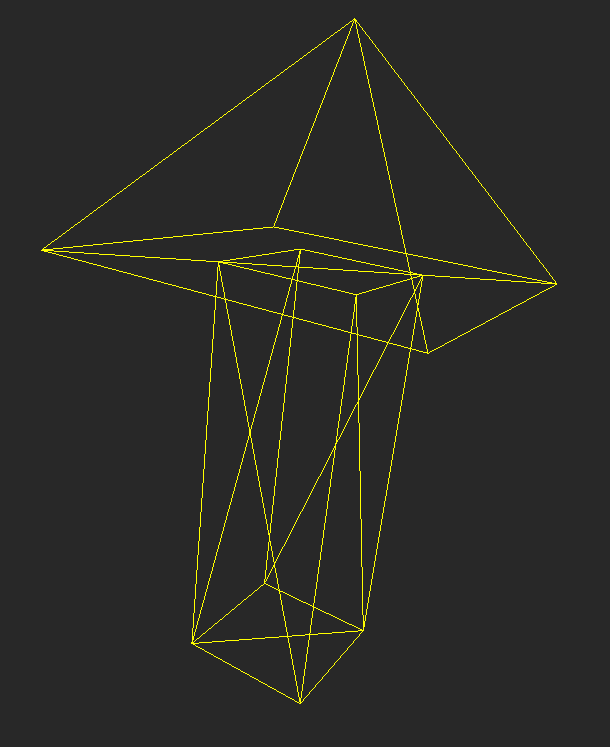
\includegraphics[width=\textwidth]{./img/4sided_arrow.PNG}
    \caption{Four-sided tip version (not used)}
    \label{fig:4sided_arrow}
	\end{subfigure}
    \qquad
    \begin{subfigure}{0.3\textwidth}
	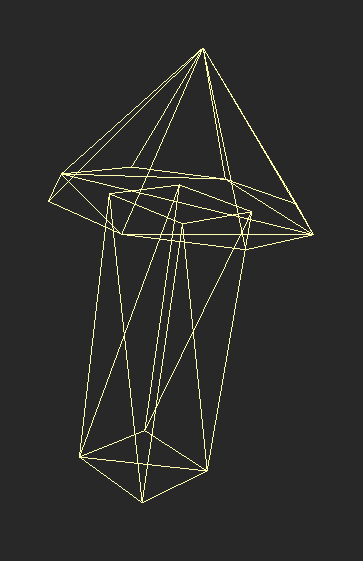
\includegraphics[width=\textwidth]{./img/8sided_arrow.PNG}
    \caption{Eight-sided tip version (used)}
    \label{fig:8sided_arrow}
	\end{subfigure}
\caption[Wireframe models used for arrow visualizations]{Wireframe models used for arrow visualizations}
\end{figure}

The visualizer receives a list of clusters as input, loops through them and makes a scaled copy of the basic arrow in each iteration. The scale of the copy is based on the representative vector of the cluster as described in section \ref{sec:analysis_visualizations}. A {\it scene} containing all the created copies is then outputted.

\subsubsection{Color Visualizers}

For each color visualization type mentioned in section \ref{sec:analysis_visualizations} (i.e. random, cluster relative, cluster absolute, etc.), there is a separate visualizer class implementing the color visualizer interface. This determines how color is assigned to vertices. In general, each visualizer loops though all \verb+Cluster+ instances supplied and for each of them it generates a color based on the metric value for that cluster. Once a color is created, it is inserted into a list at precisely those indices which belong to the \verb+PrimaryArrows+ (see section \ref{sec:implementation_clustering}) of the associated cluster in the underlying {\it scene}. It is important to respect this indexing in order to make the mapping of the colors to the mesh vertices easier in the \verb+BakeVisualization()+ method of the \verb+DiffVector+ class. This list is then outputted.

\subsubsection{Output}

Either a triangle mesh or a list of triplets representing colors is outputted based on the type of the visualization.
%%-----------------------------------------------------------------------------------------
\subsection{Visualization Output}

Lastly, we will mention how generated visualizations can be obtained through the \verb+BakeVisualization()+ method of \verb+DiffVector+ after \verb+CreateVisualization()+ has been called.

When two {\it scenes} in a specific order are provided to \verb+BakeVisualization()+, several actions might be performed based on which visualizations are available in \verb+DiffVector+:

\begin{itemize}
\item If a color visualization is available, the scenes are assumed to be the {\it primary scene} and the {\it reference scene} that the visualization was computed for, respectively, and all vertices of the scenes are assigned the corresponding color. For the {\it primary scene}, colors are assigned as they are in the visualization. For the {\it reference scene}, all colors are inverted because from the perspective of the {\it reference scene} the original metric vectors point in the opposite direction.
\item If an arrow visualization is available, the whole {\it scene} of arrows (see section \ref{sec:implementation_visualizers} for more details) is copied into the supplied {\it scenes}, where the assumed {\it reference scene} receives inverted arrows.
\item If both are available, the color visualization is baked first because the number of colors and {\it scene} vertices would not match after the arrow visualization was baked.
\end{itemize}

It is noteworthy that in the second case, there are no assumptions on the supplied {\it scene}, therefore it can be empty, in which case arrows are stored separately from the underlying {\it scene} for greater flexibility, or it can be either the {\it primary} or the {\it reference} scene, in which case everything is stored in one data structure.

Because both the {\it primary scene} and the {\it reference scene} are assigned a visualization, they can be displayed next to each other in order to emphasize the effect of the visualization. We will talk about this and the overall architecture of MeshDiff in the next chapter.
%%-----------------------------------------------------------------------------------------
%% SECTION
%%-----------------------------------------------------------------------------------------
\section{MeshDiff Architecture}

When introducing the design of MeshDiff, we will first discuss the original code by Josef Pelikán used for mesh viewing and how we modified it, then we will describe how the user interface has been changed to support features outlined in section \ref{sec:meshdiff_features} and then we will show how the visualization algorithm has been incorporated into the program.

%%-----------------------------------------------------------------------------------------
\subsection{Triangle Mesh Viewing}

The original code of MeshDiff support the two most common standard triangle mesh formats, \verb+.obj+ and \verb+.ply+. It is able to load and store files of these formats and also convert between them and the internal representation (see section \ref{sec:mesh_representation}) of a triangle mesh. This {\it scene} can then be rendered by calling its own method which fills the vertex buffer object with its data. In each frame, a special rendering method is called which comprises OpenTK calls tied to a WinForms control showing the triangle mesh. This process can be modified by a set of toggles which can change the viewing mode to wireframe or turn on shading.

Interactivity is handled by a class called \verb+Trackball+ which intercepts mouse clicks and moves from the user interface and modifies the model matrix used in the rendering process.

We have generalized this process slightly for the purpose of showing two triangle meshes at the same time. We have doubled the number of buffer objects and added parameters to the rendering methods which allow us to choose which {\it scene} to render and where to render it. Each viewing panel has its own \verb+Trackball+ and when paired control is turned on (the viewing angle and zoom of both meshes is controlled simultaneously), all mouse events are sent to both of them. This ensures that the model matrix of both triangle meshes is the same.

As mentioned in section \ref{sec:meshdiff_features}, when 3D arrows are part of the visualization, they can be stored and loaded at the same time. Also, we wanted the wireframe view toggle to work separately for arrows a that can improve the clarity of a visualization in certain cases. Therefore, we store the triangle meshes and the arrows in separate {\it scenes}. We have added one more {\it scene} parameter to the rendering methods and one more set of buffer objects to be able to implement this.
%%-----------------------------------------------------------------------------------------
\subsection{User Interface}

We have extended the original user interface by adding functionality which allows the user to configure the visualization before it is generated. The user can also save this configuration to a file or load it from a file.

There are four places in the code where this configuration is stored. The \verb+Trackball+ class remembers the model matrix and zoom value for each of the displayed triangle meshes. Currently chosen difference metric type is stored in a single variable. Clustering parameters (see section \ref{sec:parameter_effect}) have their own dedicated class and so do the visualization parameters which control the appearance of the visualizations.

Apart from being able to pass the parameters to the \verb+DiffVector+ class in a compact way, this approach also has the advantage that each class encapsulating a certain group of parameters is also able to write them to a file and it is also able to initialize itself from a file\footnotemark.

\footnotetext{Metric type is stored in a variable but there is a dedicated class called \verb+Metric+ in the program which handles metric computation and on top of that is also able to handle the input/output operations.}

Each of the parameter classes implement individual parameters as properties and handle value checks. Exceptions thrown by these checks are not being caught, however, because the user interface is designed in such a way that invalid values cannot be assigned. Invalid assignments from code are then correctly detected and an exception is thrown in such cases.
%%-----------------------------------------------------------------------------------------
\subsection{Visualization Infrastructure}

Once the user has finished their configuration and starts the visualization generation, an asynchronous job is initialized to handle this process in a user-friendly way.

The complete configuration including the visualizer classes (see section \ref{sec:implementation_visualizers}) and {\it scenes} for the triangle meshes potentially receiving new vertex colors and for potential 3D arrows become part of a job configuration package. Once a job is initialized with this package, its behavior is fully determined and its \verb+Run()+ method can be assigned to a thread. A job operates directly with the \verb+DiffVector+ class, initializes it and calls its method according to the parameters passed to it. The thread is started together with a dialog window which shows progress and at the same time prevents the user from doing anything else with the program. Once the visualization process finishes, the program checks whether is has finished successfully or not and assigns the currently displayed {\it scenes} accordingly.

-----------------------------------------

-----------------------------------------
%%-----------------------------------------------------------------------------------------
%% SECTION
%%-----------------------------------------------------------------------------------------
\section{MeshDiff Application}

In this section we will briefly talk about the main development decision behind the MeshDiff application.

Our intention is to create an experimental application which will allow us to demonstrate the proposed visualizations, conduct a user study and also provide basic features for users who wish to experiment with visualizing their own data and potentially publish the visualizations without any extra implementation work.

Just like in MeshLab or Morphome3cs, in MeshDiff, the core functionality is the ability to load and store triangle meshes and to view them interactively using the mouse cursor. Because this functionality is present in almost all programs which work with triangle meshes and at the same time it is non-trivial, we will reuse available code which provides it, more specifically we will build MeshDiff on top of a mesh viewer application written by Josef Pelikán.

%%-----------------------------------------------------------------------------------------
\subsection{Features}
\label{sec:meshdiff_features}

We will now briefly mention the features of Mesh Diff related to mesh difference visualization and the rationale behind them.

\subsubsection{Two Viewing Panels}

MeshDiff contains two viewing panels, therefore two triangle meshes can be loaded next to each other at the same time. This makes the difference visualizations much more powerful and clear because the user can see what the difference is related to.

We have also added an option for the user to control the viewing angle and zoom of both meshes at the same time. Thanks to this feature, it is easier to find the same area of interest in both meshes and examine it further.

\begin{figure}[h]
\centering
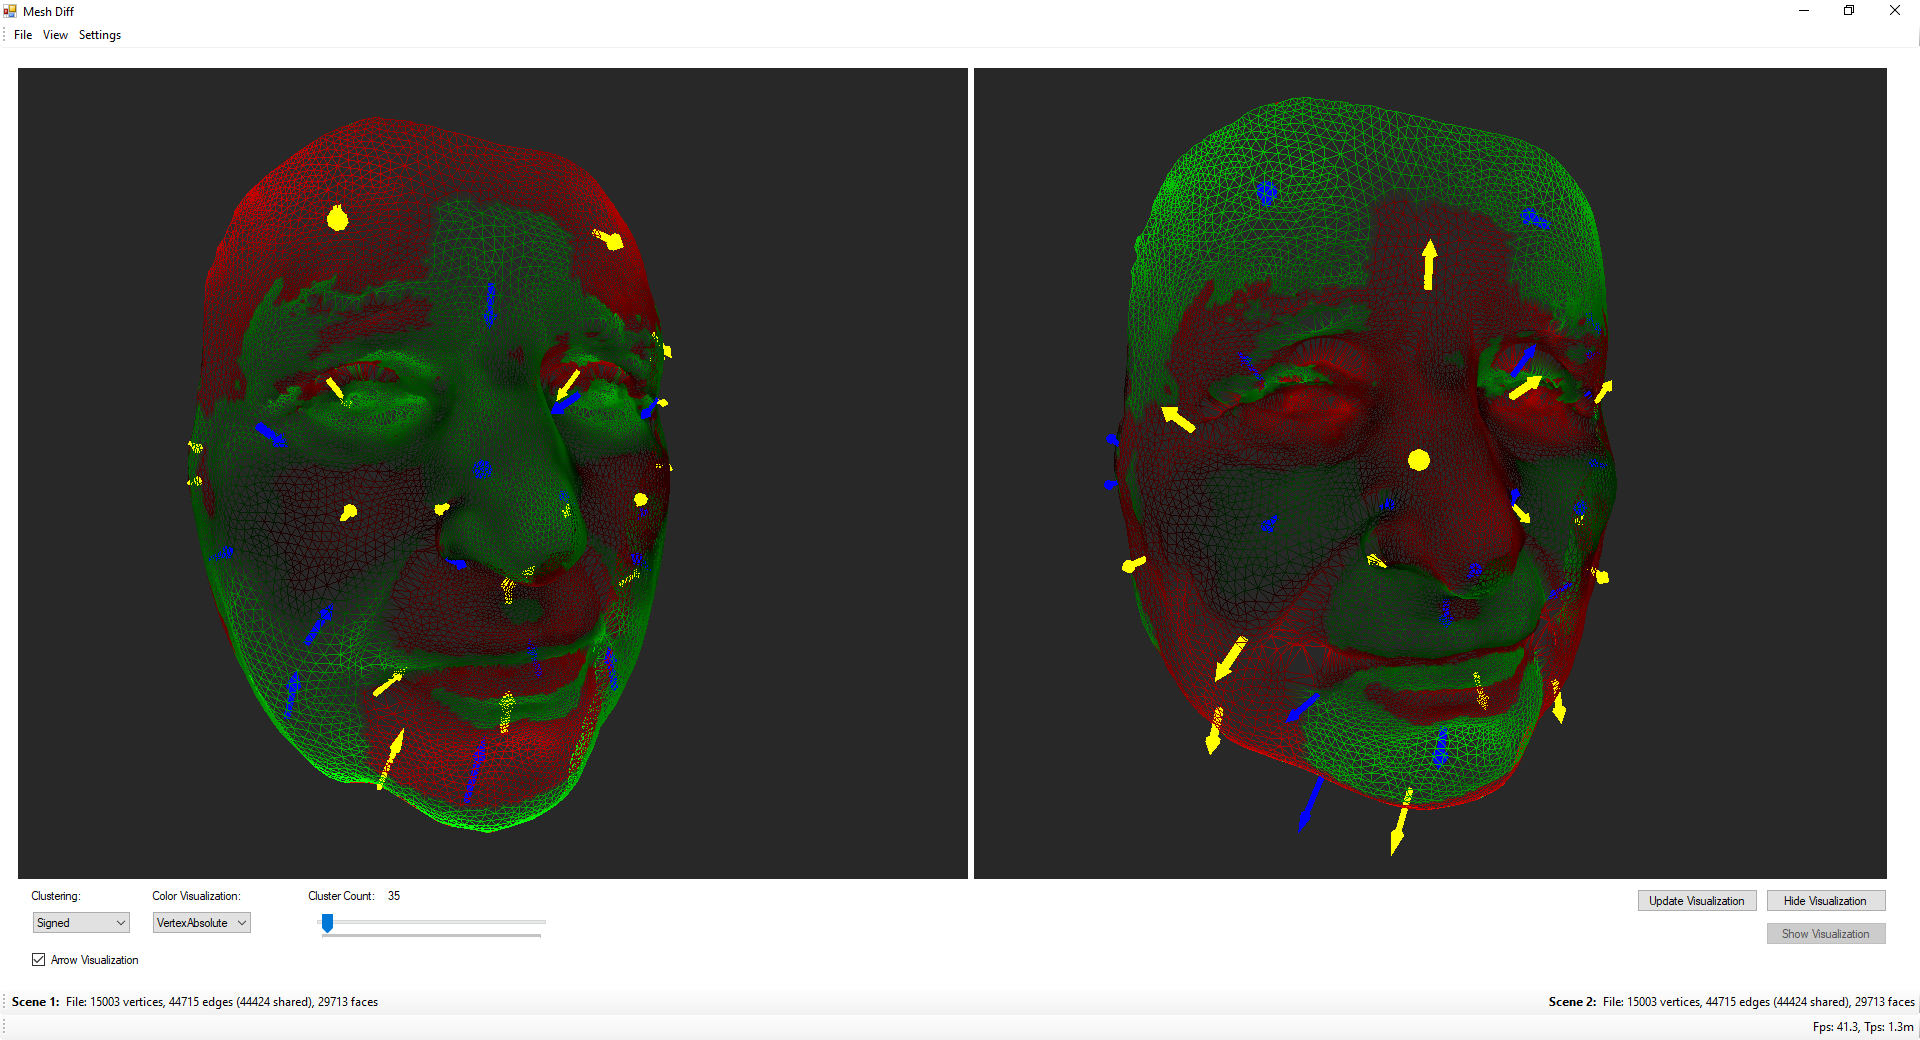
\includegraphics[width=\textwidth]{./img/meshdiff.PNG}
\caption[MeshDiff - Application view]{MeshDiff - Application view}
\label{fig:meshdiff}
\end{figure}

\subsubsection{Visualization Configuration and Generation}

The difference metric to be used, all clustering parameters (see section \ref{sec:parameter_effect}), visualization parameters (arrow size and color, thresholding, etc.) and the chosen visualization type form a configuration of the visualization process. This configuration can be fully customized in the user interface where the user can also generate a visualization and then toggle its visibility. Such a feature is vital for the full demonstration of the proposed methods.

\subsubsection{Visualization Store and Load}

Mesh Diff supports loading and storing of visualizations in the standard \verb+.ply+ format. This format was chosen because it is able to store color in vertices which makes it easier to work with than for example \verb+.obj+ where additional textures would have to be used for storing color. 

In arrow visualizations (see section\ref{sec:arrow_vis}), the mesh and the arrows  can be stored in separate \verb+.ply+ files and also loaded from them which increases the variability of the application.

\subsubsection{Configuration Store and Load}

The complete configuration including the viewing angle and zoom value of both triangle meshes can also be saved to a file and subsequently loaded. Replication, demonstration and publication of specific visualizations is much easier with this feature.
%%-----------------------------------------------------------------------------------------
\subsection{Platform}

Mesh Diff is written in C\#, its user interface is created in WinForms and rendering is handled by the OpenTK library which provides an interface to OpenGL in C\#. The reason for this choice is that we have available code written by Josef Pelikán which supports exactly those features that were mentioned at the beginning of this section and is easily extensible to support the extra features we have outlined above. Because MeshDiff is mainly of experimental nature and is mostly meant for the demonstration of visualization algorithms, the only targeted operating system is Windows.